\documentclass[12pt,a4paper]{article}

\usepackage[T1]{fontenc}
\usepackage[utf8]{inputenc}
\usepackage[serbian]{babel}
\usepackage{lmodern}
\usepackage{microtype}
\usepackage{geometry}
\geometry{margin=2.4cm}
\usepackage{graphicx}
\usepackage{booktabs}
\usepackage{tabularx}
\usepackage{array}
\usepackage{caption}
\usepackage{subcaption}
\usepackage{enumitem}
\usepackage{hyperref}
\usepackage{setspace}
\usepackage{fancyhdr}
\usepackage{listings}
\usepackage{xcolor}

\hypersetup{
  colorlinks=true,
  linkcolor=black,
  urlcolor=blue!60!black,
  citecolor=black
}

\onehalfspacing
\setlength{\parskip}{0.45em}
\setlength{\parindent}{0pt}

\pagestyle{fancy}
\fancyhf{}
\fancyhead[L]{\small Mašinsko učenje --- MFUB}
\fancyhead[R]{\small avgust 2026.}
\fancyfoot[C]{\thepage}
\renewcommand{\headrulewidth}{0.4pt}

\lstset{
  basicstyle=\ttfamily\small,
  breaklines=true,
  frame=single,
  backgroundcolor=\color{gray!8},
  rulecolor=\color{gray!40}
}

\captionsetup{font=small,labelfont=bf}

\begin{document}

\begin{titlepage}
  \centering
  \vspace*{1.5cm}
  {\Large Matematički fakultet\par}
  {\large Univerzitet u Beogradu\par}
  \vspace{2cm}
  {\huge\bfseries Prepoznavanje umetničkih pokreta\\pomoću dubokih CNN mreža\par}
  \vspace{1.5cm}
  {\large Predmet: Mašinsko učenje\par}
  \vspace{2.5cm}
  {\large
    Anja Jovanović, 1044/2025\\
    Mateja Stojanović, 1107/2025\par}
  \vfill
  {\large Beograd, avgust 2026.\par}
\end{titlepage}

\begin{abstract}
\noindent
Rad se bavi klasifikacijom slika umetničkih dela u jedan od 18 umetničkih pokreta na skupu Pandora 18K.
Testirali smo četiri modela: dve konvolucione mreže trenirane od nule (VGG-lite i hibrid sa Inception-stil granom)
i transfer learning sa InceptionV3, prvo sa novom dense glavom, a zatim sa fine-tuningom poslednjeg konvolucionog bloka.
Najbolji rezultat dao je fine-tune model: test accuracy 56{,}91\% i macro F1 0{,}570.
To je u skladu sa rezultatima iz literature za isti zadatak.
Custom modeli su ostali znatno ispod toga (VGG-lite 35{,}14\%, hibrid 27{,}72\%),
što pokazuje koliko pomaže prethodno učenje na ImageNet-u.

\medskip
\noindent\textbf{Ključne reči:} CNN, transfer learning, fine-tuning, klasifikacija slika, umetnički pokreti, Pandora 18K
\end{abstract}

\tableofcontents
\newpage

\section{Uvod}

Kad gledamo sliku u galeriji, lako uočimo da li je reč o impresionizmu, kubizmu ili pop artu,
ali je teško objasniti koji od pravaca je u pitanju ako se ne zna tačan autor slike.
Model ne traži objekat na slici, već način slikanja: potez, boju, kompoziciju, stepen apstrakcije.
Zato je prepoznavanje umetničkog pokreta teži zadatak od klasične klasifikacije,
posebno kad su dva pokreta bliska i po vremenu i po izgledu.

Skup Pandora 18K sadrži 18\,038 slika u 18 klasa, od vizantijske ikonografije do pop arta.
U ovom projektu smo na tom skupu uporedili mreže koje učimo od nule i pristup zasnovan na pretreniranoj InceptionV3 mreži.

Cilj nam je bio da vidimo koliko dobijamo samim treniranjem male CNN arhitekture,
koliko pomaže zamena poslednjeg sloja na već naučenoj mreži,
i da li ima smisla pustiti da se prilagodi još jedan konvolucioni blok.
Sve smo radili na istoj podeli podataka, da bi poređenje bilo pravedno.

\section{Srodni radovi}

Florea, Toca i Gieske su uveli Pandora 18K i pokazali da se stilovi mogu razlikovati i klasičnim metodama,
kombinacijom boje i topografskih deskriptora sa boosting-om.
To je dobar polazni kontekst, ali duboke mreže na većem broju klasa daju drugačije rezultate.

Yu, Jin i Hsu su na istom skupu testirali VGG-lite, hibridnu arhitekturu i transfer learning sa InceptionV3.
Njihov VGG-lite je imao oko 31\% tačnosti, hibrid oko 36\%, a transfer sa fine-tuningom oko 56 do 57\%.
Mi smo se držali slične postavke eksperimenata da bismo mogli da uporedimo brojeve.

Transfer learning je standardan kad ima malo podataka u novom domenu.
Zamrzne se veći deo mreže naučene na ImageNet-u, doda nova glava za naše klase,
pa se eventualno odmrzne poslednji deo mreže malim learning rate-om.
Za InceptionV3 ulaz je obično $299\times 299$ piksela,
sa predprocesiranjem koje očekuje opseg vrednosti od $-1$ do $1$.

\section{Skup podataka}

\subsection{Pandora 18K: poreklo i struktura}

Pandora 18K je javno dostupan skup slika umetničkih dela koji su uveli Florea, Toca i Gieske.
Slike su prikupljene sa interneta i organizovane po umetničkom pokretu, zatim po autoru.
Tipična putanja izgleda ovako:

\begin{lstlisting}
Pandora_18k/09_Impressionism/Claude Monet/impression-sunrise.jpg
Pandora_18k/18_PopArt/Andy Warhol/campbell-soup.jpg
\end{lstlisting}

Autori skupa traže da se dataset citira u radovima koji ga koriste.
Slike su namenjene za istraživanje i mašinsko učenje, a ne za komercijalnu upotrebu van akademskog konteksta.

U projektu koristimo 18 klasa, hronološki od vizantijske ikonografije do pop arta:

\begin{table}[htbp]
  \centering
  \caption{Broj slika po klasi u skupu Pandora 18K}
  \label{tab:classes}
  \small
  \begin{tabular}{clr}
    \toprule
    Br. & Klasa & Broj slika \\
    \midrule
    01 & Vizantijska ikonografija & 847 \\
    02 & Rana renesansa & 751 \\
    03 & Severna renesansa & 821 \\
    04 & Visoka renesansa & 832 \\
    05 & Barok & 990 \\
    06 & Rokoko & 832 \\
    07 & Romantizam & 895 \\
    08 & Realizam & 1\,199 \\
    09 & Impresionizam & 1\,257 \\
    10 & Postimpresionizam & 1\,276 \\
    11 & Ekspresionizam & 1\,027 \\
    12 & Simbolizam & 1\,057 \\
    13 & Fovizam & 719 \\
    14 & Kubizam & 1\,227 \\
    15 & Surrealizam & 1\,072 \\
    16 & Apstraktna umetnost & 1\,063 \\
    17 & Naivna umetnost & 1\,053 \\
    18 & Pop art & 1\,120 \\
    \midrule
    \multicolumn{2}{r}{Ukupno} & 18\,038 \\
    \bottomrule
  \end{tabular}
\end{table}

Najveća klasa je postimpresionizam (1\,276), najmanja fovizam (719).
Odnos je oko 1{,}8 prema 1. Skup nije savršeno balansiran, ali nije ni ekstremno neravnomeran.

\subsection{EDA: šta smo primetili na skupu}

Pre treniranja smo pregledali podatke u \texttt{notebooks/01\_eda.ipynb}.

\paragraph{Broj slika po klasi.}
Realizam, impresionizam, postimpresionizam i kubizam imaju više od 1\,200 primera.
Manje zastupljeni su fovizam, rana renesansa i vizantijska ikonografija.

\begin{figure}[htbp]
  \centering
  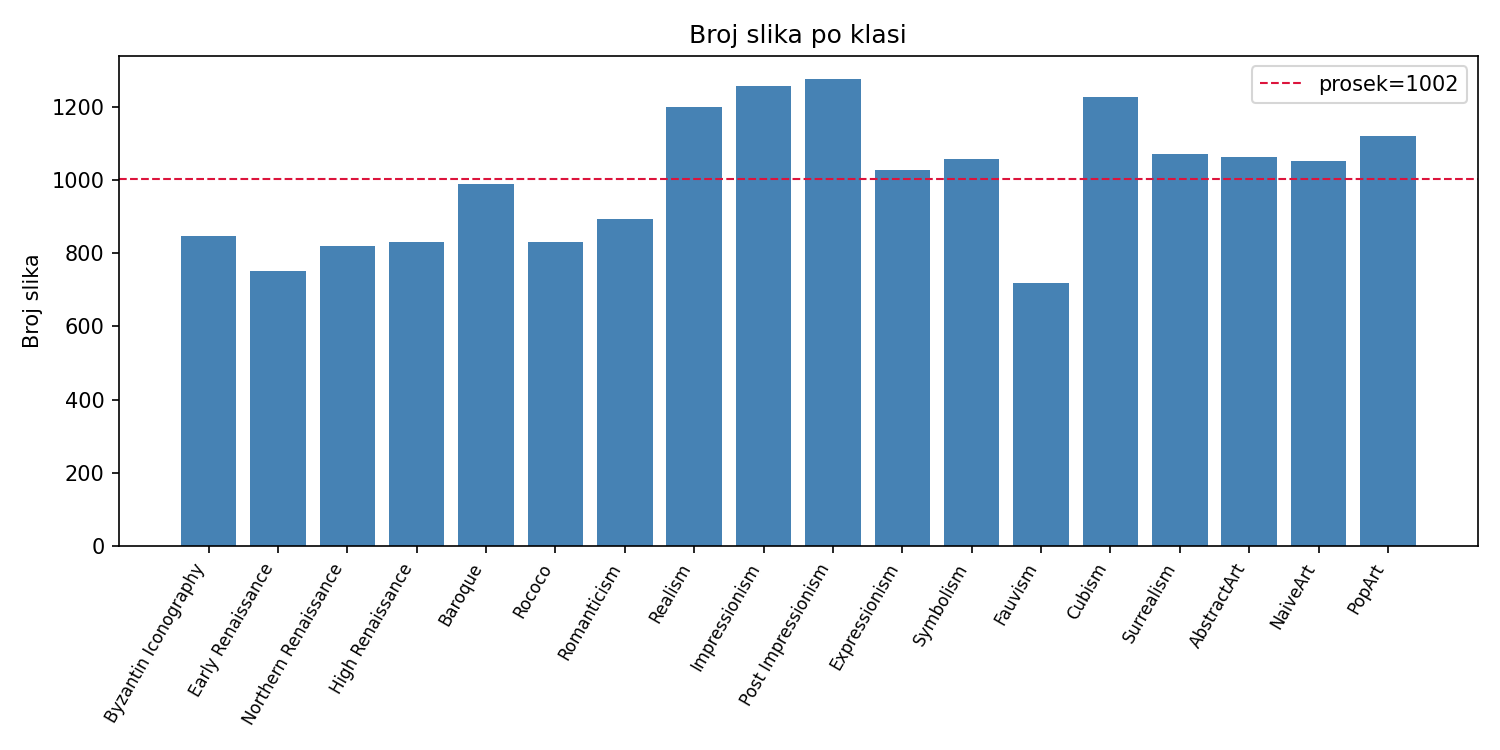
\includegraphics[width=0.92\textwidth]{figures/class_counts.png}
  \caption{Broj slika po klasi}
  \label{fig:class_countspng}
\end{figure}

\paragraph{Dimenzije slika.}
Širina i visina jako variraju. Ima malih skenova i velikih reprodukcija (preko 3\,000 piksela).
Zato sve slike skaliramo na fiksnu veličinu ($224\times 224$ za custom modele, $299\times 299$ za InceptionV3).

\begin{figure}[htbp]
  \centering
  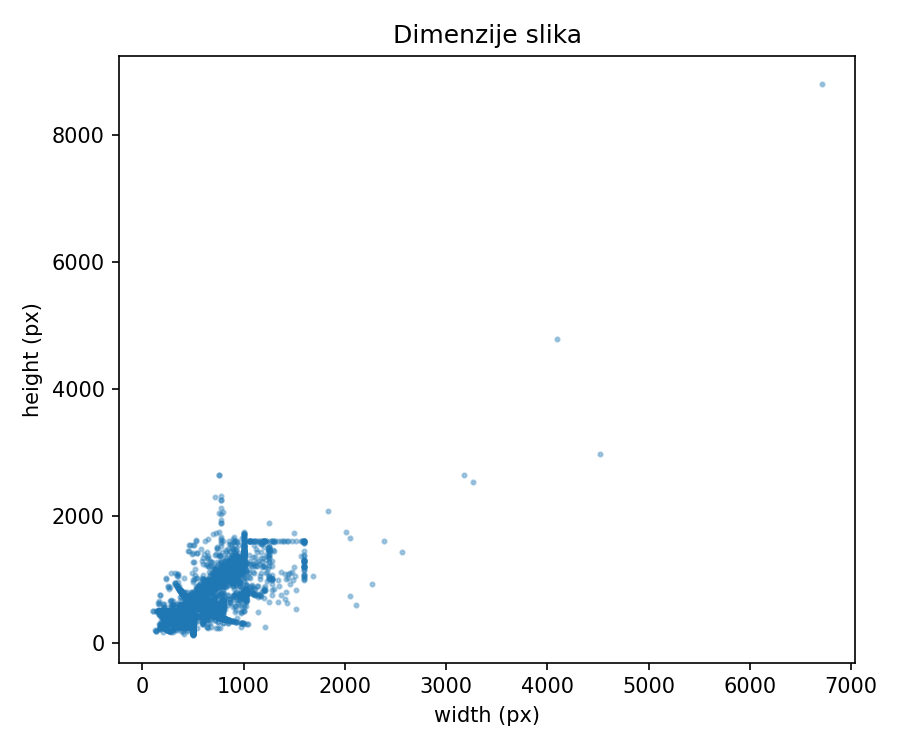
\includegraphics[width=0.78\textwidth]{figures/size_scatter.png}
  \caption{Rasip dijagram širine i visine slika}
  \label{fig:size_scatterpng}
\end{figure}

\begin{figure}[htbp]
  \centering
  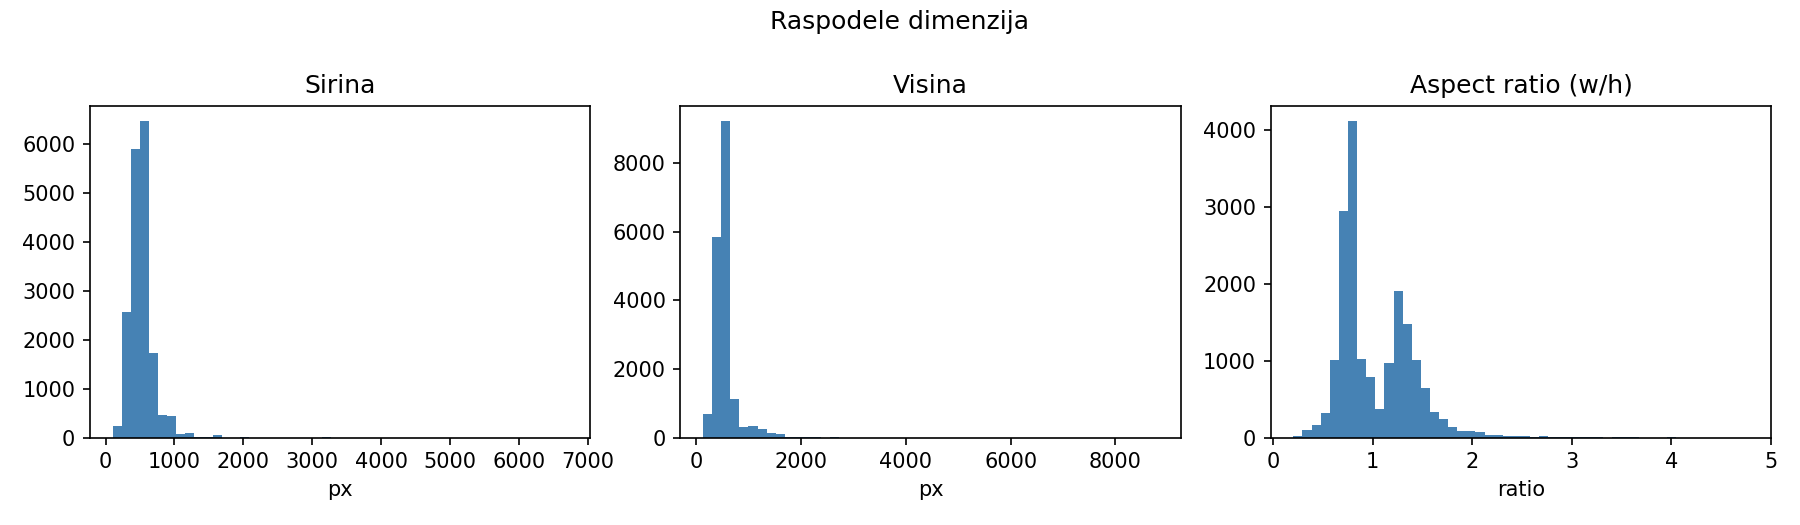
\includegraphics[width=0.92\textwidth]{figures/size_histograms.png}
  \caption{Histogrami dimenzija slika}
  \label{fig:size_histogramspng}
\end{figure}

\paragraph{Vizuelni uzorci.}
Na mreži od po jedne slike po klasi odmah se vidi razlika između, recimo, vizantijske ikonografije i pop arta.
Ali i srodni pokreti deluju slično: impresionizam i postimpresionizam dele svetlu paletu i labav potez.

\begin{figure}[htbp]
  \centering
  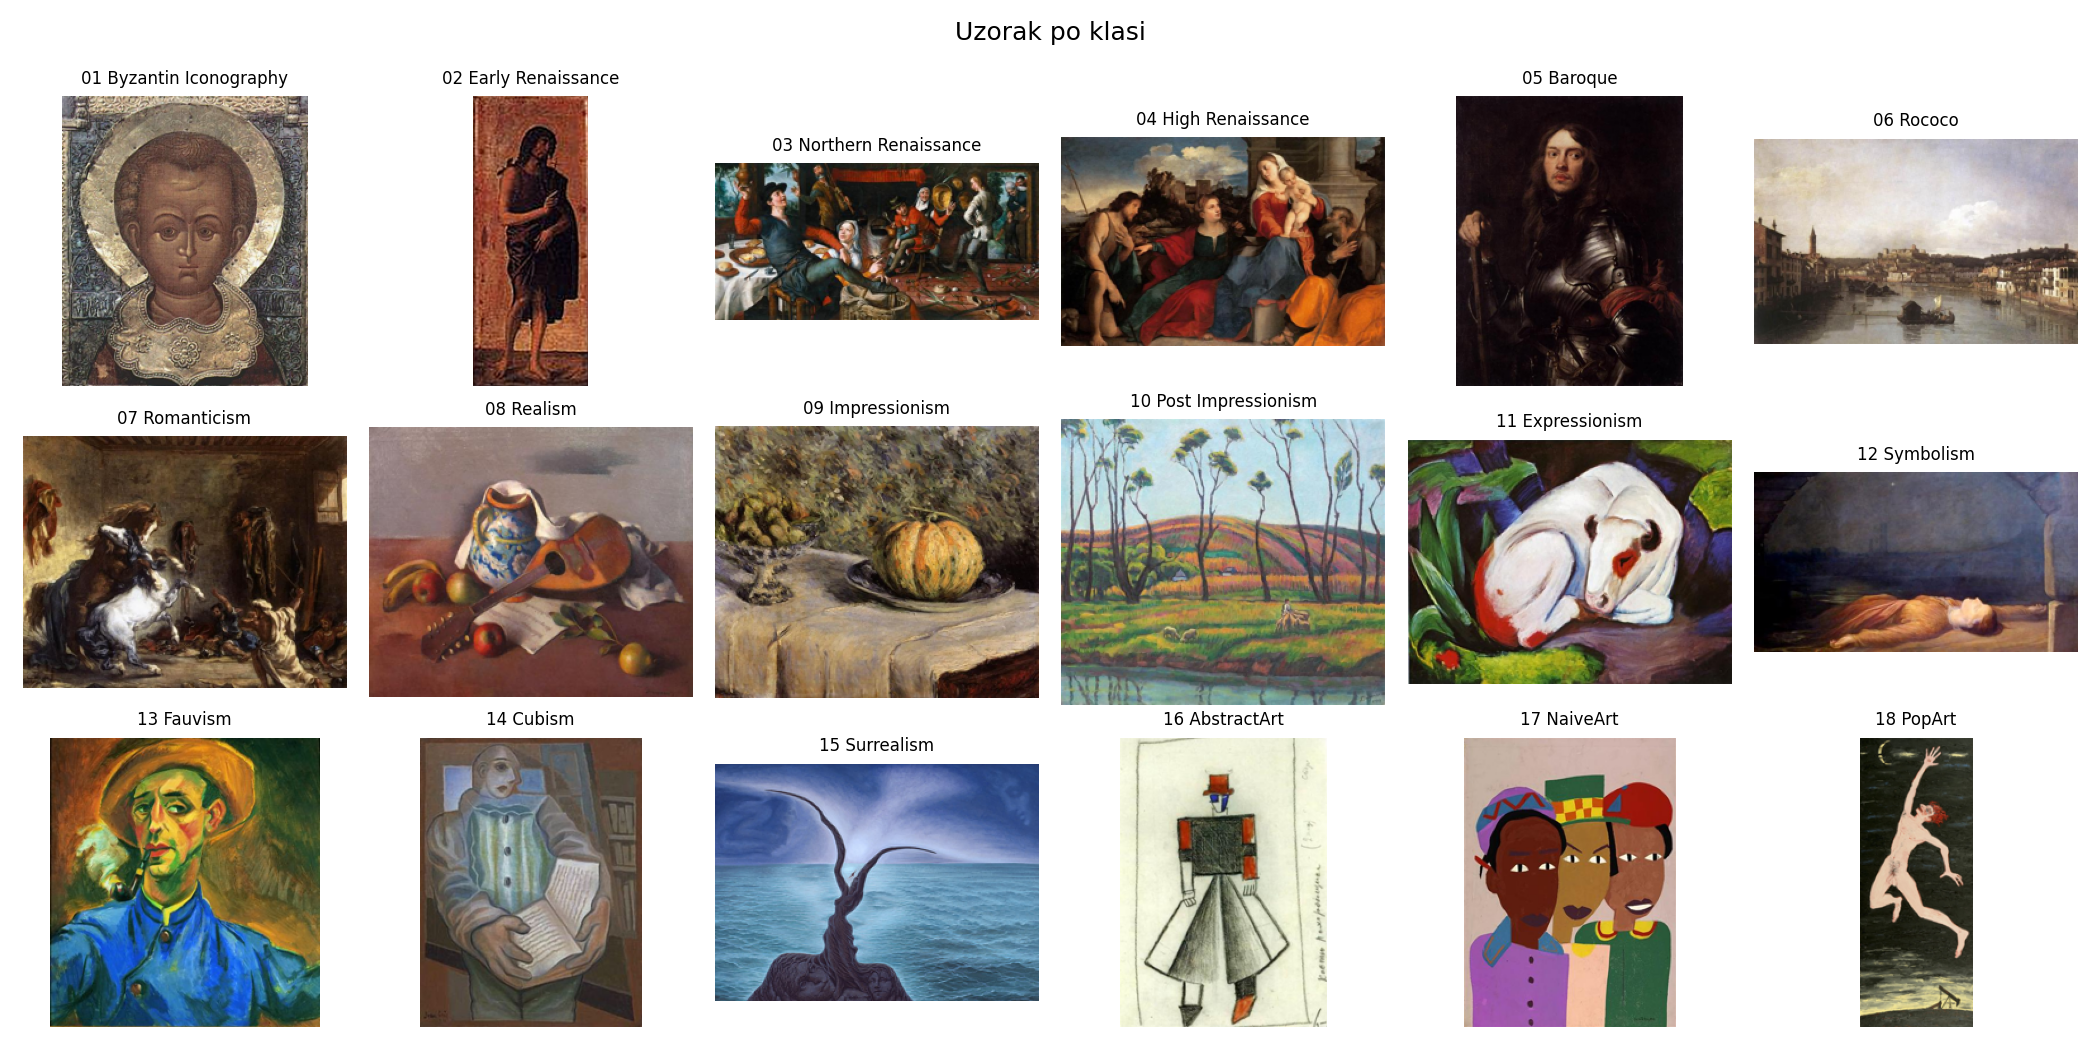
\includegraphics[width=\textwidth]{figures/sample_grid.png}
  \caption{Uzorak po jednoj slici iz svake klase}
  \label{fig:sample_gridpng}
\end{figure}

\paragraph{Struktura foldera.}
Pošto su slike grupisane po autoru unutar pokreta, isti stil se ponavlja na mnogo slika istog slikara.
Model može da nauči i specifičnosti autora, ne samo pokreta.

\subsection{Podela na trening, validaciju i test}

\begin{table}[htbp]
  \centering
  \caption{Stratifikovana podela skupa Pandora 18K}
  \label{tab:split}
  \begin{tabular}{lrr}
    \toprule
    Skup & Broj slika & Udeo \\
    \midrule
    Trening    & 12\,626 & 70\% \\
    Validacija &  2\,706 & 15\% \\
    Test       &  2\,706 & 15\% \\
    \midrule
    \textbf{Ukupno} & \textbf{18\,038} & \textbf{100\%} \\
    \bottomrule
  \end{tabular}
\end{table}

Podela je stratifikovana po klasi (\texttt{SEED = 42}).
Liste putanja su u \texttt{data/splits/train.csv}, \texttt{val.csv} i \texttt{test.csv}.
Test skup nismo koristili tokom podešavanja modela.
Na trening skupu smo uključili blagu augmentaciju (horizontalno preslikavanje, rotacija do $10^\circ$, zoom do 10\%).
Za 18 klasa nasumično pogađanje daje 5{,}56\% tačnosti.

\section{Metode}

\subsection{Custom CNN modeli}

\subsubsection{VGG-lite}
Počeli smo od jednostavne VGG-inspirisane mreže sa četiri bloka (Conv3$\times$3 + MaxPooling),
filterima 32/64/128/256, GlobalAveragePooling, Dense(256), Dropout 0{,}5 i softmax izlazom.
Ulaz: $224\times 224$, Adam lr 0{,}001, 20 epoha, batch 64. Model ima 1\,242\,674 parametara.

\subsubsection{Hibrid (Inception-stil)}
Tanji stem (8/16/32/64) i jedna Inception-stil grana sa paralelnim putanjama 1$\times$1, 3$\times$3 i 5$\times$5.
Isti ulaz i 20 epoha; hibrid treniran sa batch 128. Model ima 57\,434 parametra.

\subsection{Transfer learning sa dense glavom}
InceptionV3 sa ImageNet težinama, zamrznuta baza, nova glava (GAP + Dropout + Dense).
Ulaz $299\times 299$. Feature keš u \texttt{experiments/transfer\_dense/features/}.
100 epoha, batch 64; trenabilno 36\,882 od 21\,839\,666 parametara.

\subsection{Fine-tuning poslednjeg bloka}
Odmrznut poslednji Inception blok (\texttt{mixed9}), lr $10^{-5}$, do 30 epoha (early stopping na 28).
Trenabilno 6\,107\,154 parametara.

\subsection{Evaluacija}
Sve modele evaluirali smo skriptom \texttt{src/evaluate.py} na test skupu od 2\,706 slika.
Čuvamo model sa najboljom validacionom tačnošću (\texttt{ModelCheckpoint} po \texttt{val\_accuracy}).

\section{Rezultati}

\subsection{Uporedna tabela}

\begin{table}[htbp]
  \centering
  \caption{Uporedni rezultati svih modela}
  \label{tab:results}
  \small
  \begin{tabular}{lrrrrrrr}
    \toprule
    Model & Parametara & Trenabilnih & Ulaz & Epoha & Val acc & Test acc & Macro F1 \\
    \midrule
    VGG-lite           & 1\,242\,674  & 1\,242\,674 & $224^2$ & 20  & 33{,}85\% & 35{,}14\% & 0{,}330 \\
    Hibrid             &     57\,434  &     57\,434 & $224^2$ & 20  & 28{,}09\% & 27{,}72\% & 0{,}238 \\
    Transfer dense     & 21\,839\,666 &     36\,882 & $299^2$ & 100 & 52{,}77\% & 49{,}93\% & 0{,}497 \\
    Transfer fine-tune & 21\,839\,666 &  6\,107\,154 & $299^2$ & 28 & 59{,}57\% & \textbf{56{,}91\%} & \textbf{0{,}570} \\
    \bottomrule
  \end{tabular}
\end{table}

Napomena: 59{,}57\% je validaciona tačnost fine-tune modela; glavni rezultat je test accuracy 56{,}91\%.

\begin{figure}[htbp]
  \centering
  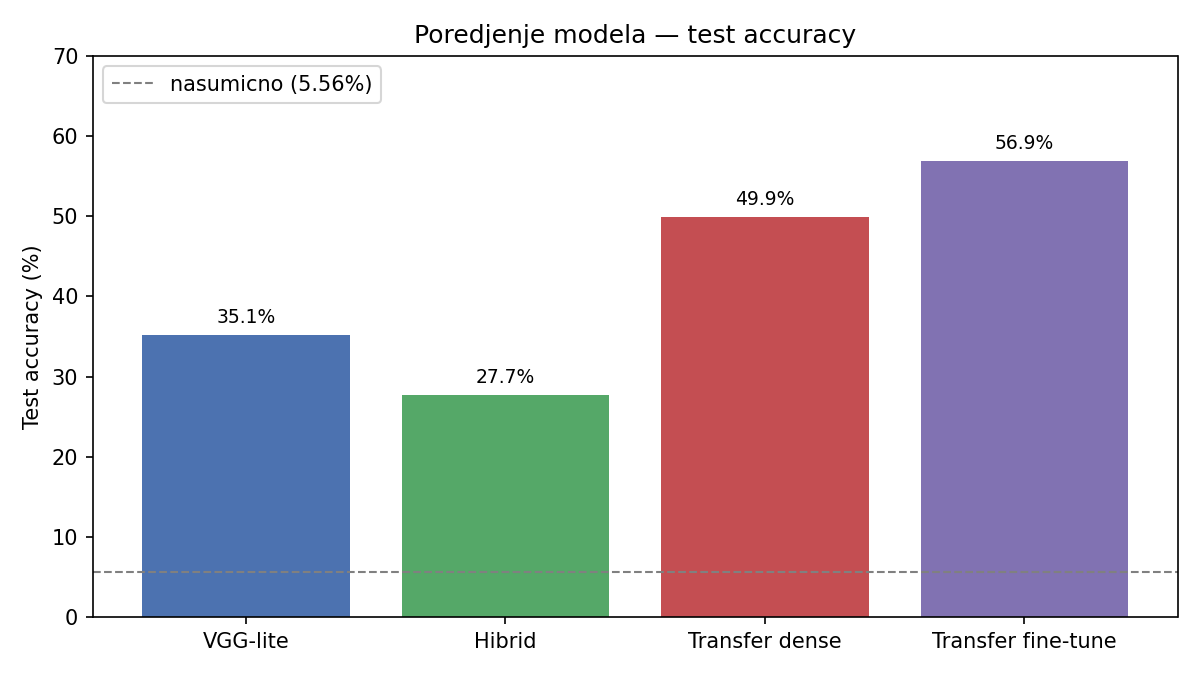
\includegraphics[width=0.85\textwidth]{figures/model_comparison_test_acc.png}
  \caption{Poređenje modela po test accuracy}
  \label{fig:model_comparison}
\end{figure}

\subsection{Custom modeli}

VGG-lite je dostigao 35{,}14\% na testu. Hibrid je imao 27{,}72\%, iako ima daleko manje parametara.

\begin{figure}[htbp]
  \centering
  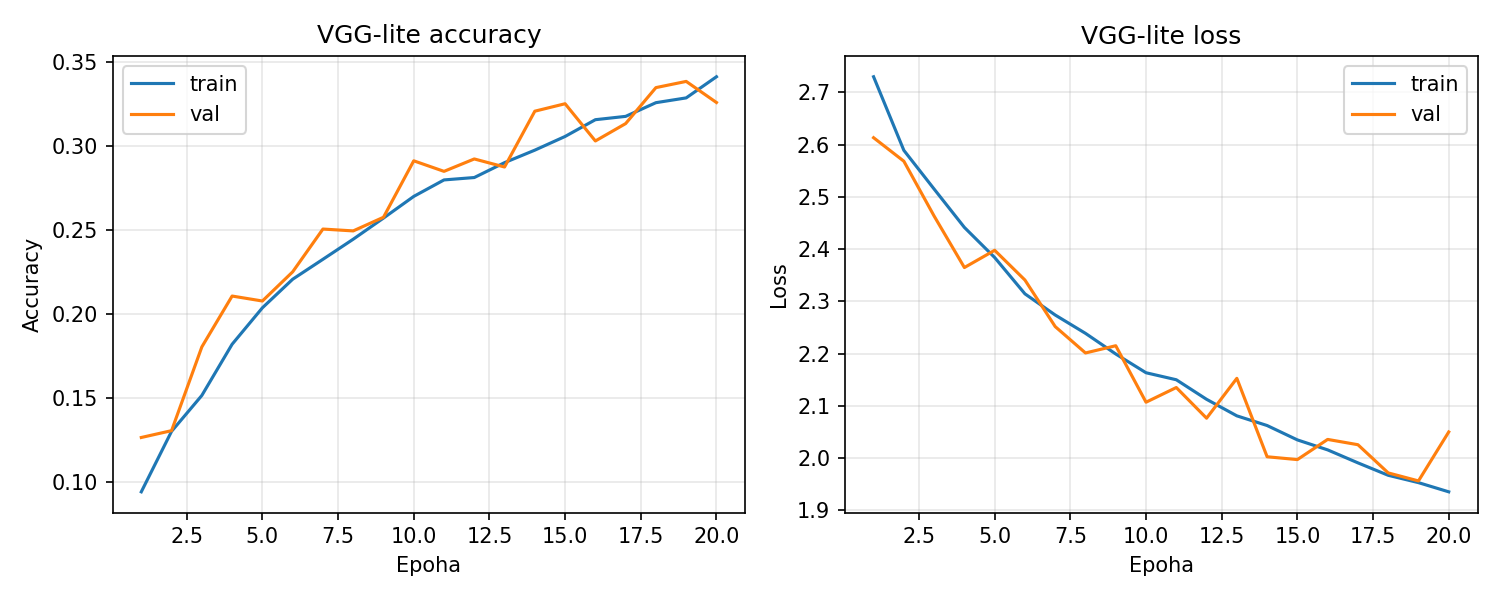
\includegraphics[width=0.95\textwidth]{figures/vgglite_curves.png}
  \caption{Krive učenja — VGG-lite}
  \label{fig:vgglite_curvespng}
\end{figure}

\begin{figure}[htbp]
  \centering
  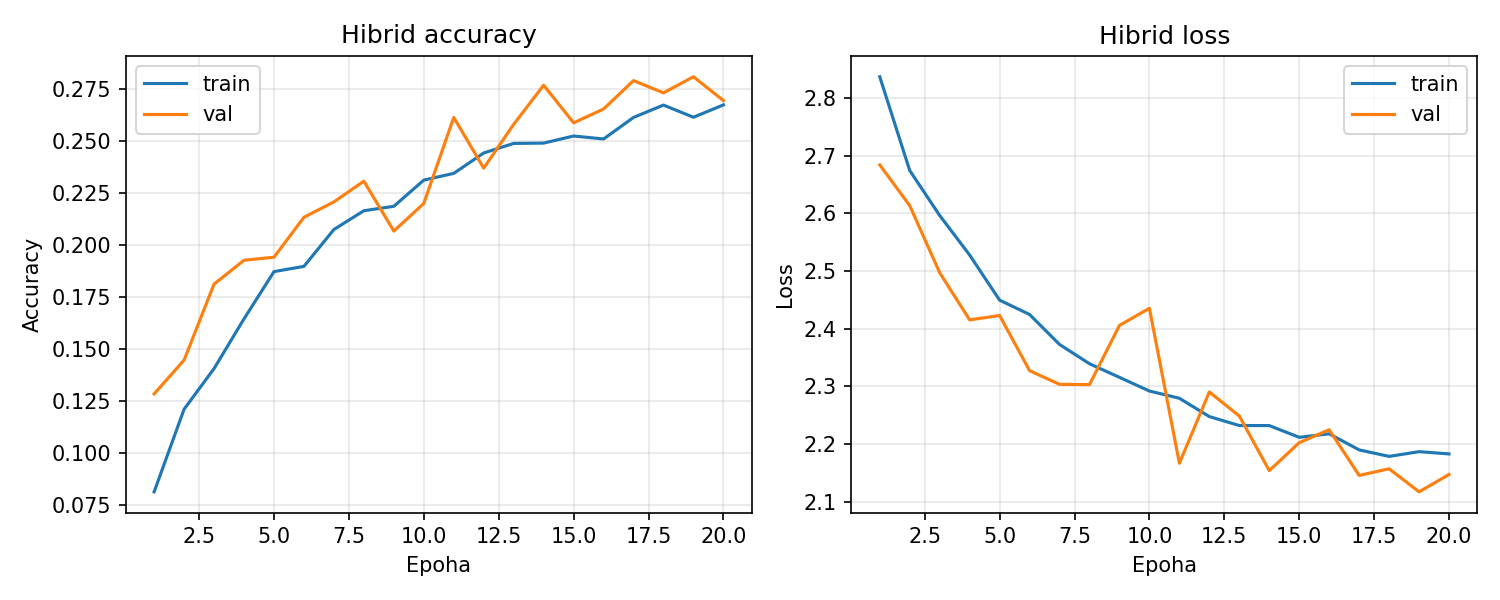
\includegraphics[width=0.95\textwidth]{figures/hybrid_curves.png}
  \caption{Krive učenja — hibrid}
  \label{fig:hybrid_curvespng}
\end{figure}

\subsection{Transfer modeli}

Dense glava daje 49{,}93\% test accuracy; fine-tuning podiže na 56{,}91\% (+6{,}98 p.p.).
Macro F1 raste sa 0{,}497 na 0{,}570.

\begin{table}[htbp]
  \centering
  \caption{Poređenje transfer dense i fine-tune modela}
  \label{tab:transfer}
  \begin{tabular}{lcc}
    \toprule
    Metrika & Transfer dense & Transfer fine-tune \\
    \midrule
    Test accuracy & 49{,}93\% & 56{,}91\% \\
    Test loss     & 1{,}4698 & 1{,}3791 \\
    Macro F1      & 0{,}4965 & 0{,}5704 \\
    Weighted F1   & 0{,}4912 & 0{,}5657 \\
    \bottomrule
  \end{tabular}
\end{table}

\begin{figure}[htbp]
  \centering
  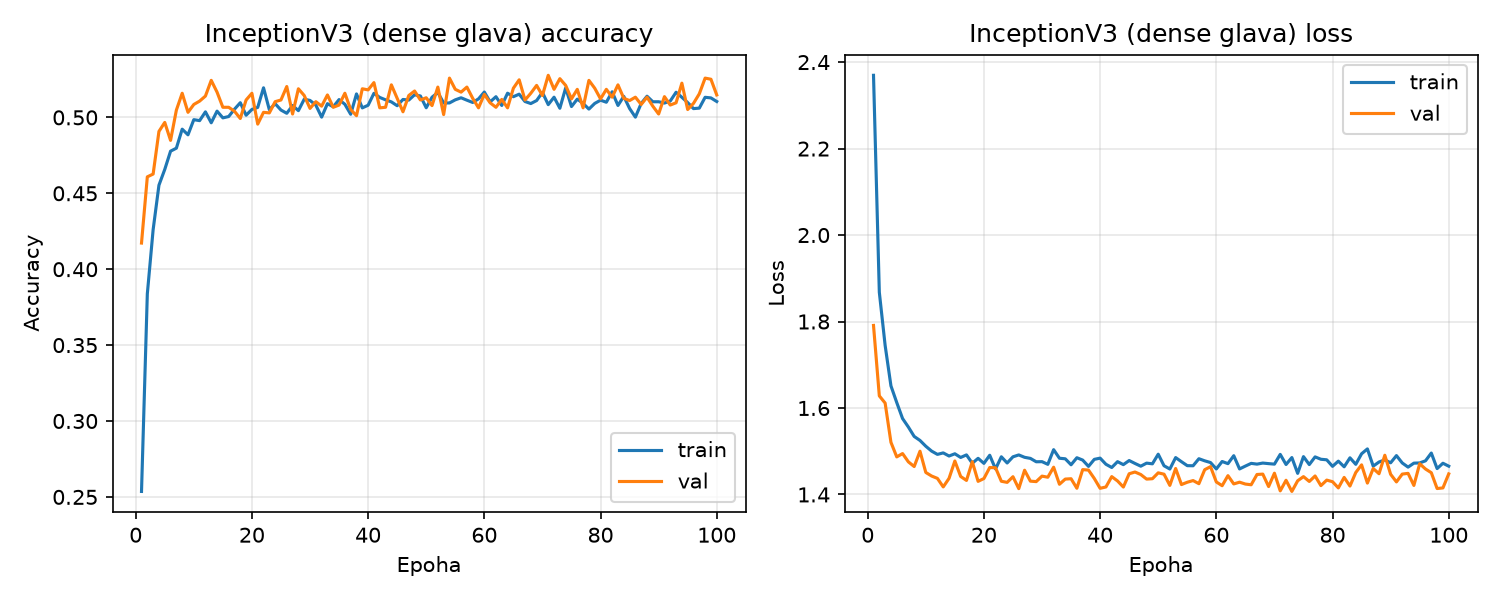
\includegraphics[width=0.95\textwidth]{figures/transfer_dense_curves.png}
  \caption{Krive učenja — transfer dense}
  \label{fig:transfer_dense_curvespng}
\end{figure}

\begin{figure}[htbp]
  \centering
  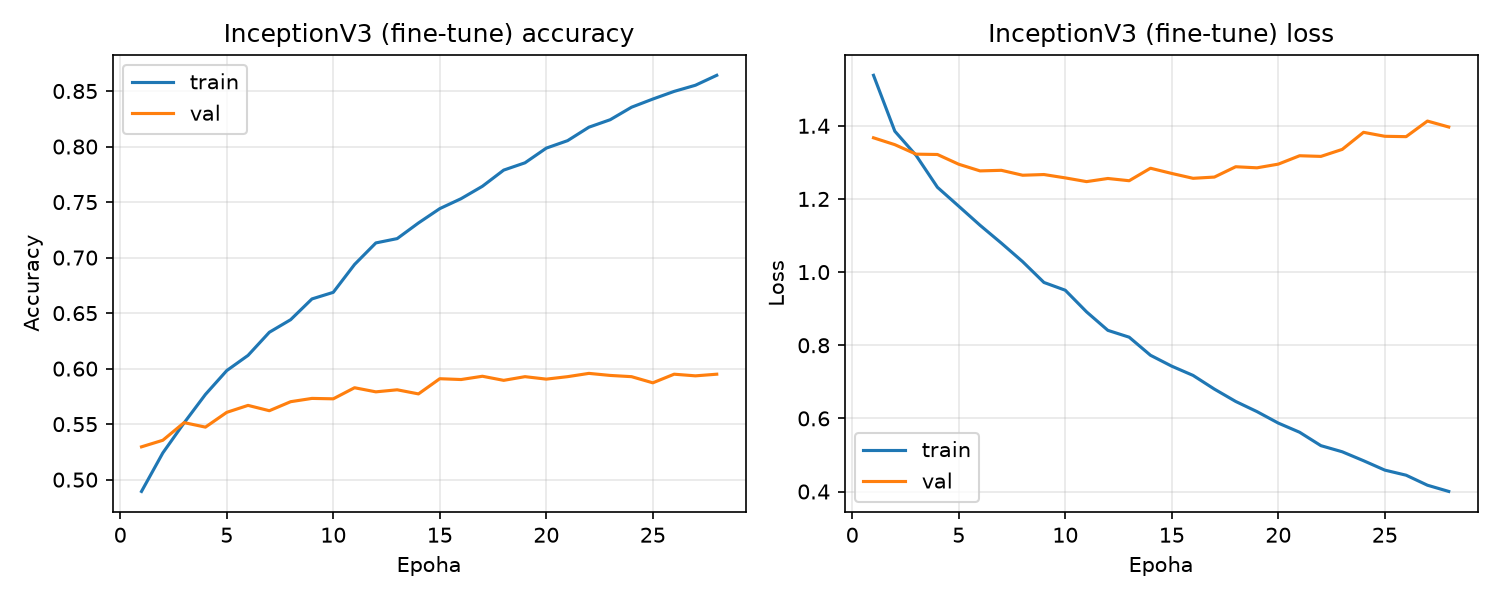
\includegraphics[width=0.95\textwidth]{figures/transfer_finetune_curves.png}
  \caption{Krive učenja — transfer fine-tune}
  \label{fig:transfer_finetune_curvespng}
\end{figure}

\begin{figure}[htbp]
  \centering
  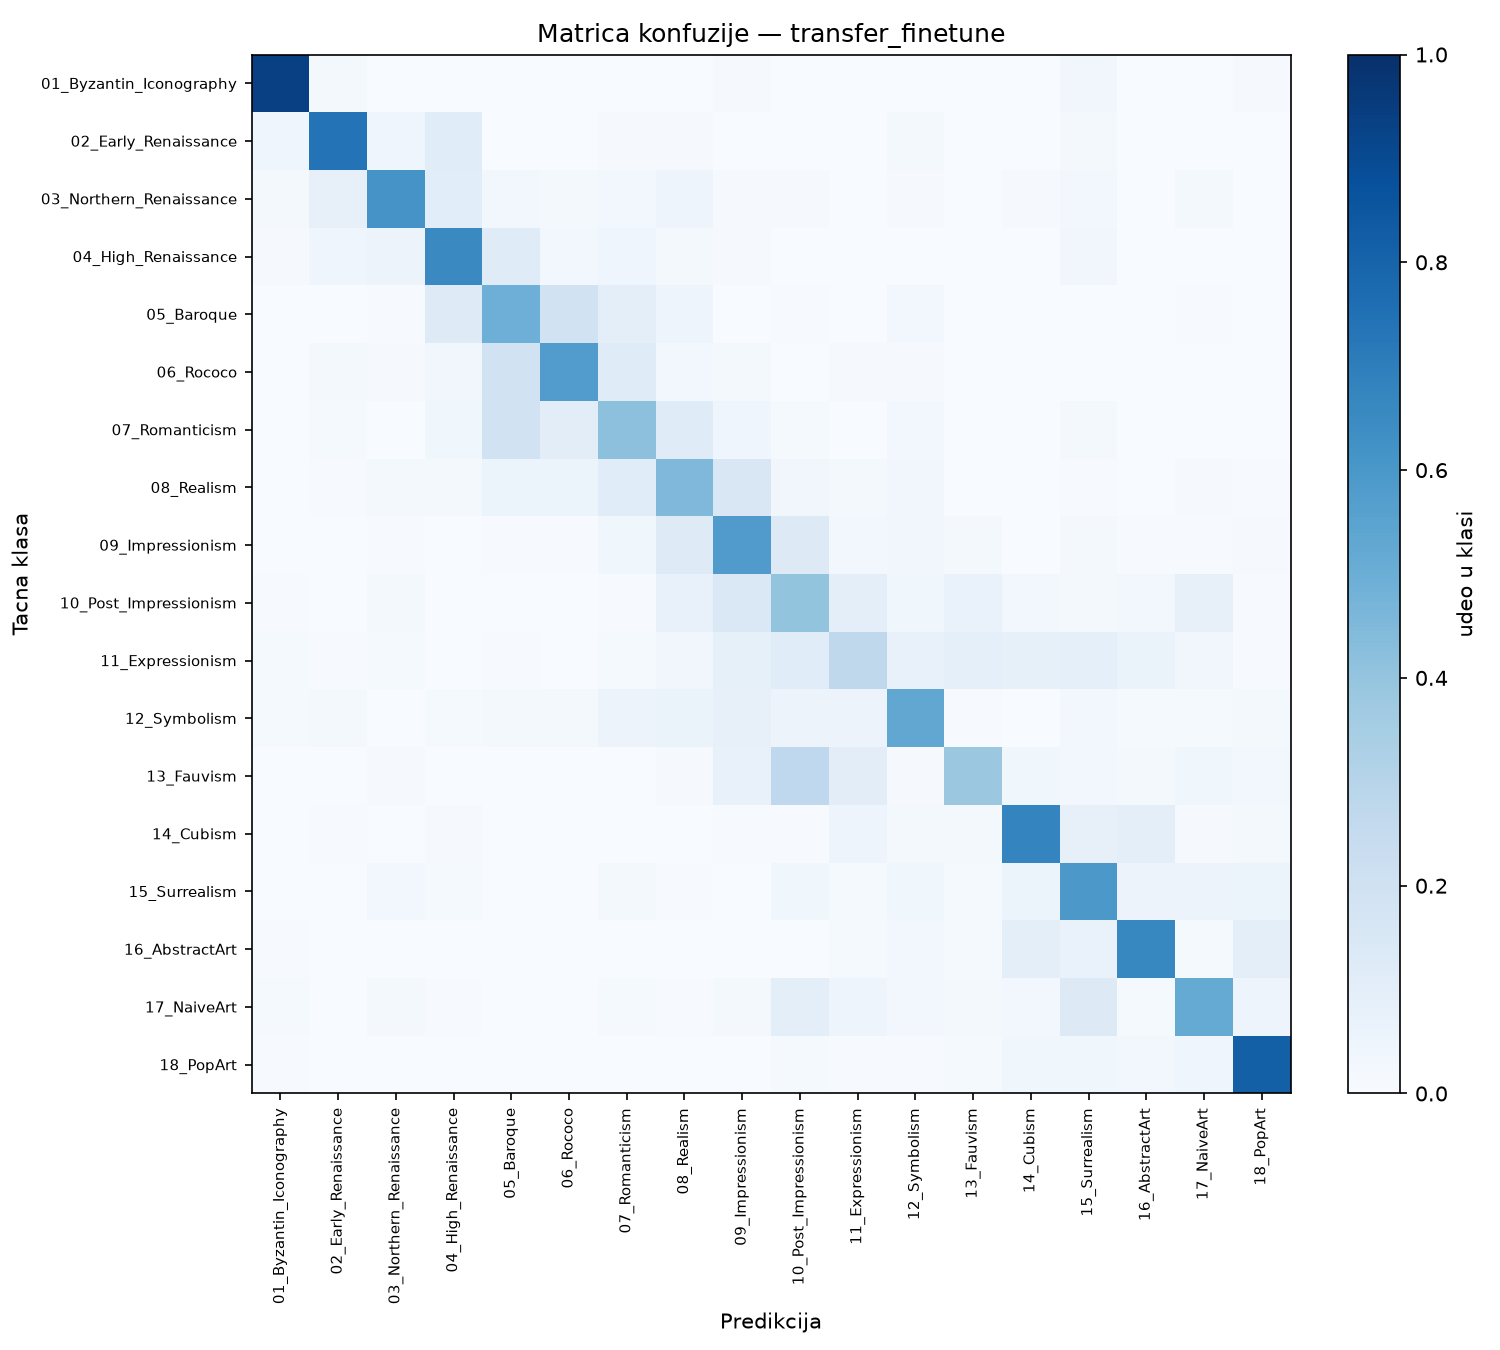
\includegraphics[width=0.88\textwidth]{figures/transfer_finetune_confusion.png}
  \caption{Matrica konfuzije — transfer fine-tune}
  \label{fig:transfer_finetune_confusionpng}
\end{figure}

\subsection{Analiza grešaka po klasama}

Analizu smo radili na najboljem modelu (transfer fine-tune).
Na test skupu od 2\,706 slika model je uredno klasifikovao 56{,}91\% slika.

\begin{table}[htbp]
  \centering
  \caption{Klase koje model najbolje prepoznaje}
  \label{tab:best-classes}
  \small
  \begin{tabular}{lrl}
    \toprule
    Klasa & Recall & Komentar \\
    \midrule
    Vizantijska ikonografija & 93{,}7\% & Zlatna pozadina, jasan stil \\
    Pop art & 81{,}5\% & Jarke boje, lako se razlikuje \\
    Rana renesansa & 74{,}1\% & Prepoznatljiva kompozicija \\
    Kubizam & 67{,}4\% & Geometrijski oblici \\
    \bottomrule
  \end{tabular}
\end{table}

\begin{table}[htbp]
  \centering
  \caption{Klase koje model najčešće pogrešno klasifikuje}
  \label{tab:worst-classes}
  \small
  \begin{tabular}{lrrl}
    \toprule
    Klasa & Recall & Precision & Problem \\
    \midrule
    Ekspresionizam & 27{,}3\% & 0{,}38 & Meša se sa postimpresionizmom \\
    Postimpresionizam & 40{,}1\% & 0{,}40 & Često ide u impresionizam \\
    Romantizam & 41{,}8\% & 0{,}40 & Meša se sa barokom \\
    Barok & 49{,}3\% & 0{,}46 & Zbunjuje ga sa rokokoom \\
    Realizam & 45{,}0\% & 0{,}47 & Često kao impresionizam \\
    \bottomrule
  \end{tabular}
\end{table}

\begin{table}[htbp]
  \centering
  \caption{Najčešće zabune između parova klasa}
  \label{tab:confusions}
  \small
  \begin{tabular}{llr}
    \toprule
    Tačna klasa & Pogrešno predviđeno kao & Broj slika \\
    \midrule
    Fovizam & Postimpresionizam & 29 \\
    Postimpresionizam & Impresionizam & 28 \\
    Barok & Rokoko & 28 \\
    Realizam & Impresionizam & 27 \\
    Romantizam & Barok & 26 \\
    Impresionizam & Postimpresionizam & 24 \\
    Rokoko & Barok & 24 \\
    Realizam & Romantizam & 21 \\
    Naivna umetnost & Surrealizam & 20 \\
    Ekspresionizam & Postimpresionizam & 18 \\
    Kubizam & Apstraktna umetnost & 18 \\
    \bottomrule
  \end{tabular}
\end{table}

Većina grešaka nije nasumična, već je koncentrisana oko istorijski i vizuelno srodnih pokreta.

\begin{enumerate}[leftmargin=*, itemsep=0.35em]
  \item \textbf{Postimpresionizam predviđen kao impresionizam} --- slična svetla paleta i potez.
  \item \textbf{Realizam predviđen kao impresionizam} --- meki prelazi i difuzno svetlo.
  \item \textbf{Romantizam predviđen kao barok} --- dramatično svetlo i kontrasti.
  \item \textbf{Ekspresionizam predviđen kao postimpresionizam} --- subjektivni izraz forme.
  \item \textbf{Fovizam predviđen kao postimpresionizam} --- jarke boje; manje primera u skupu.
\end{enumerate}

\begin{figure}[htbp]
  \centering
  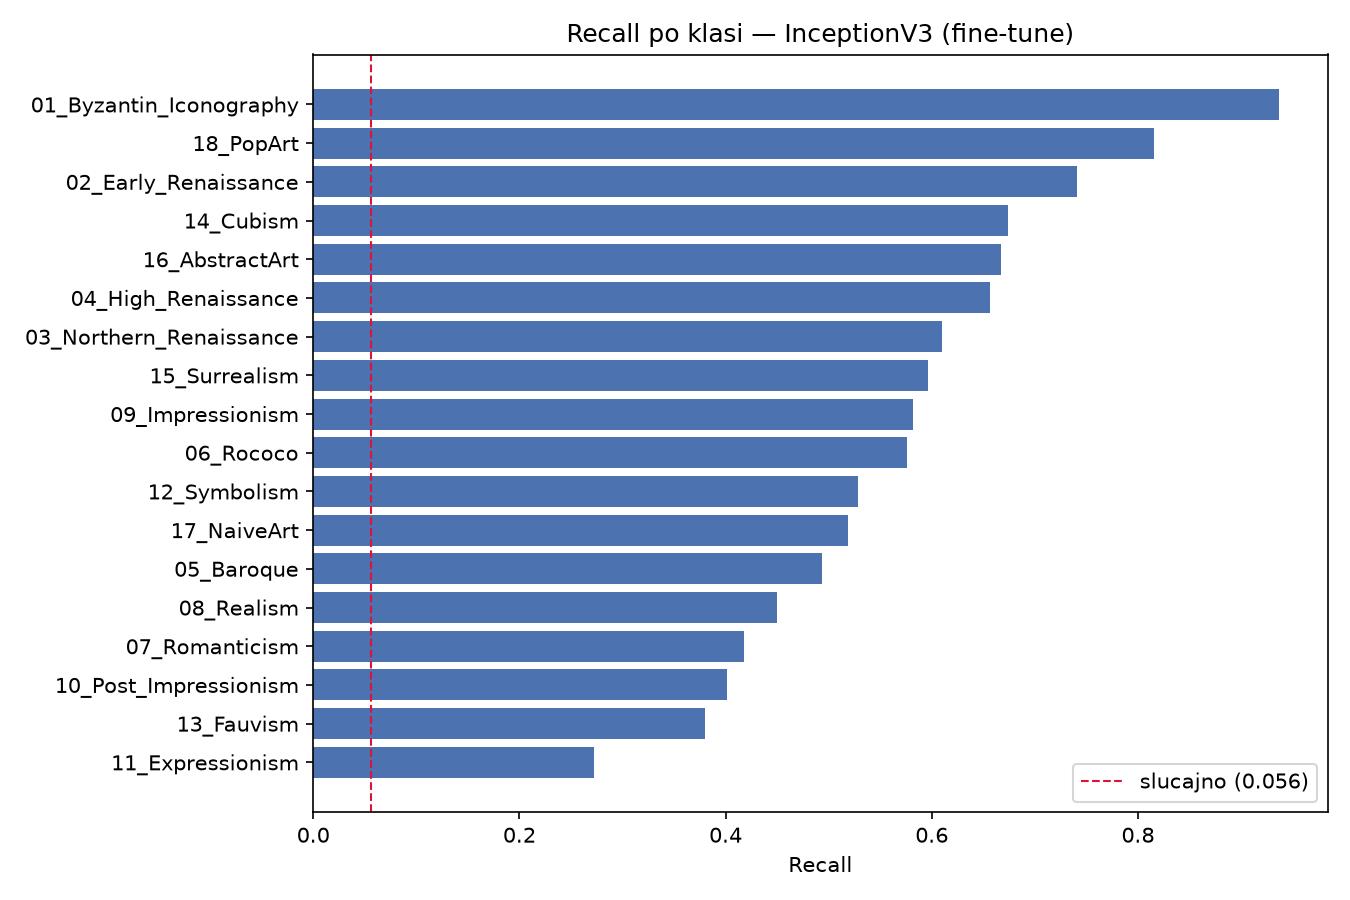
\includegraphics[width=0.92\textwidth]{figures/transfer_finetune_recall_per_class.png}
  \caption{Recall po klasi — transfer fine-tune}
  \label{fig:transfer_finetune_recall_per_classpng}
\end{figure}

\begin{figure}[htbp]
  \centering
  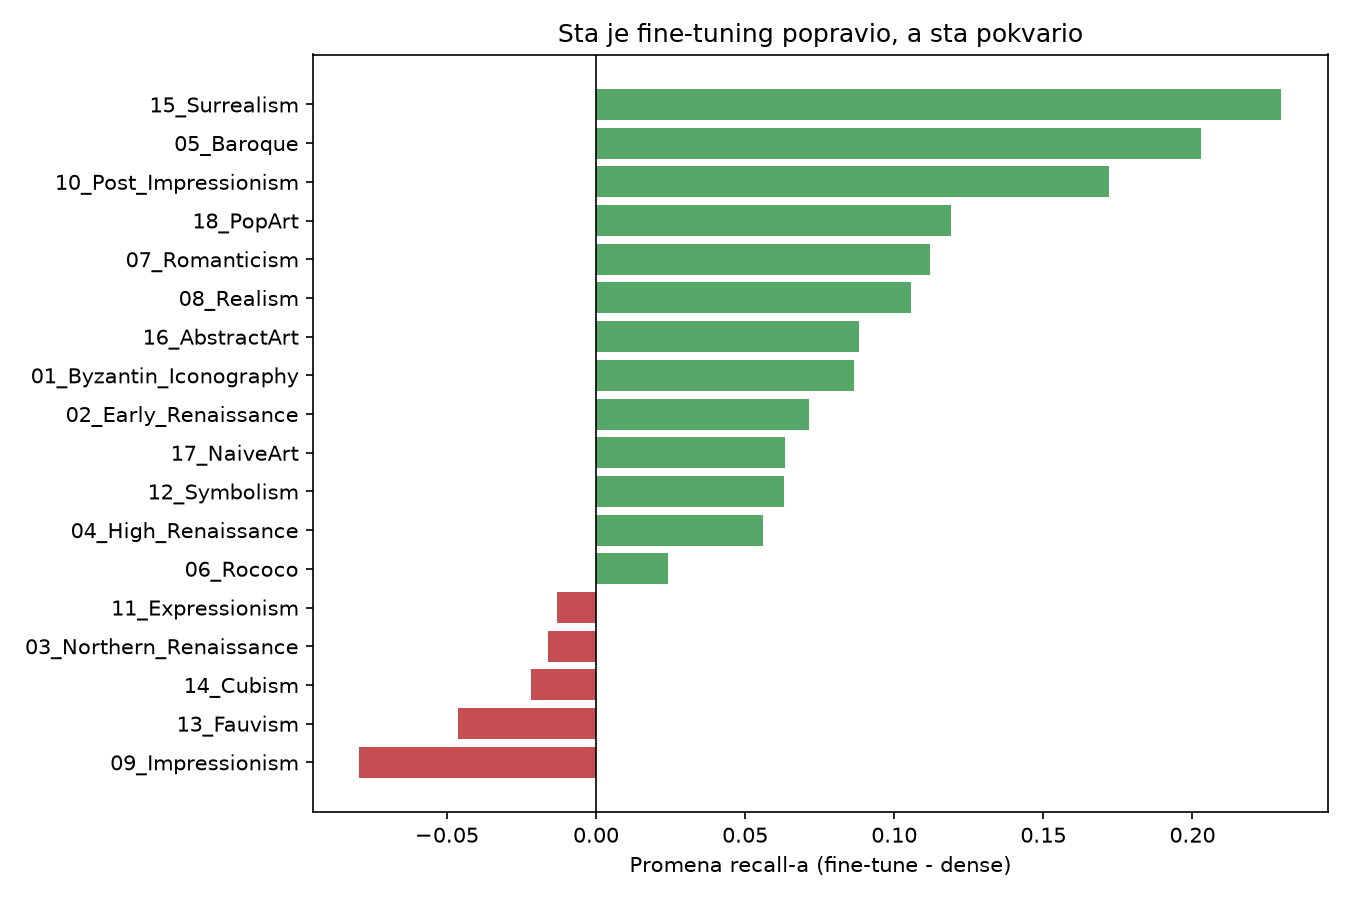
\includegraphics[width=0.92\textwidth]{figures/transfer_finetune_vs_dense_recall.png}
  \caption{Poređenje recall-a: dense vs fine-tune}
  \label{fig:transfer_finetune_vs_dense_recallpng}
\end{figure}

\begin{figure}[htbp]
  \centering
  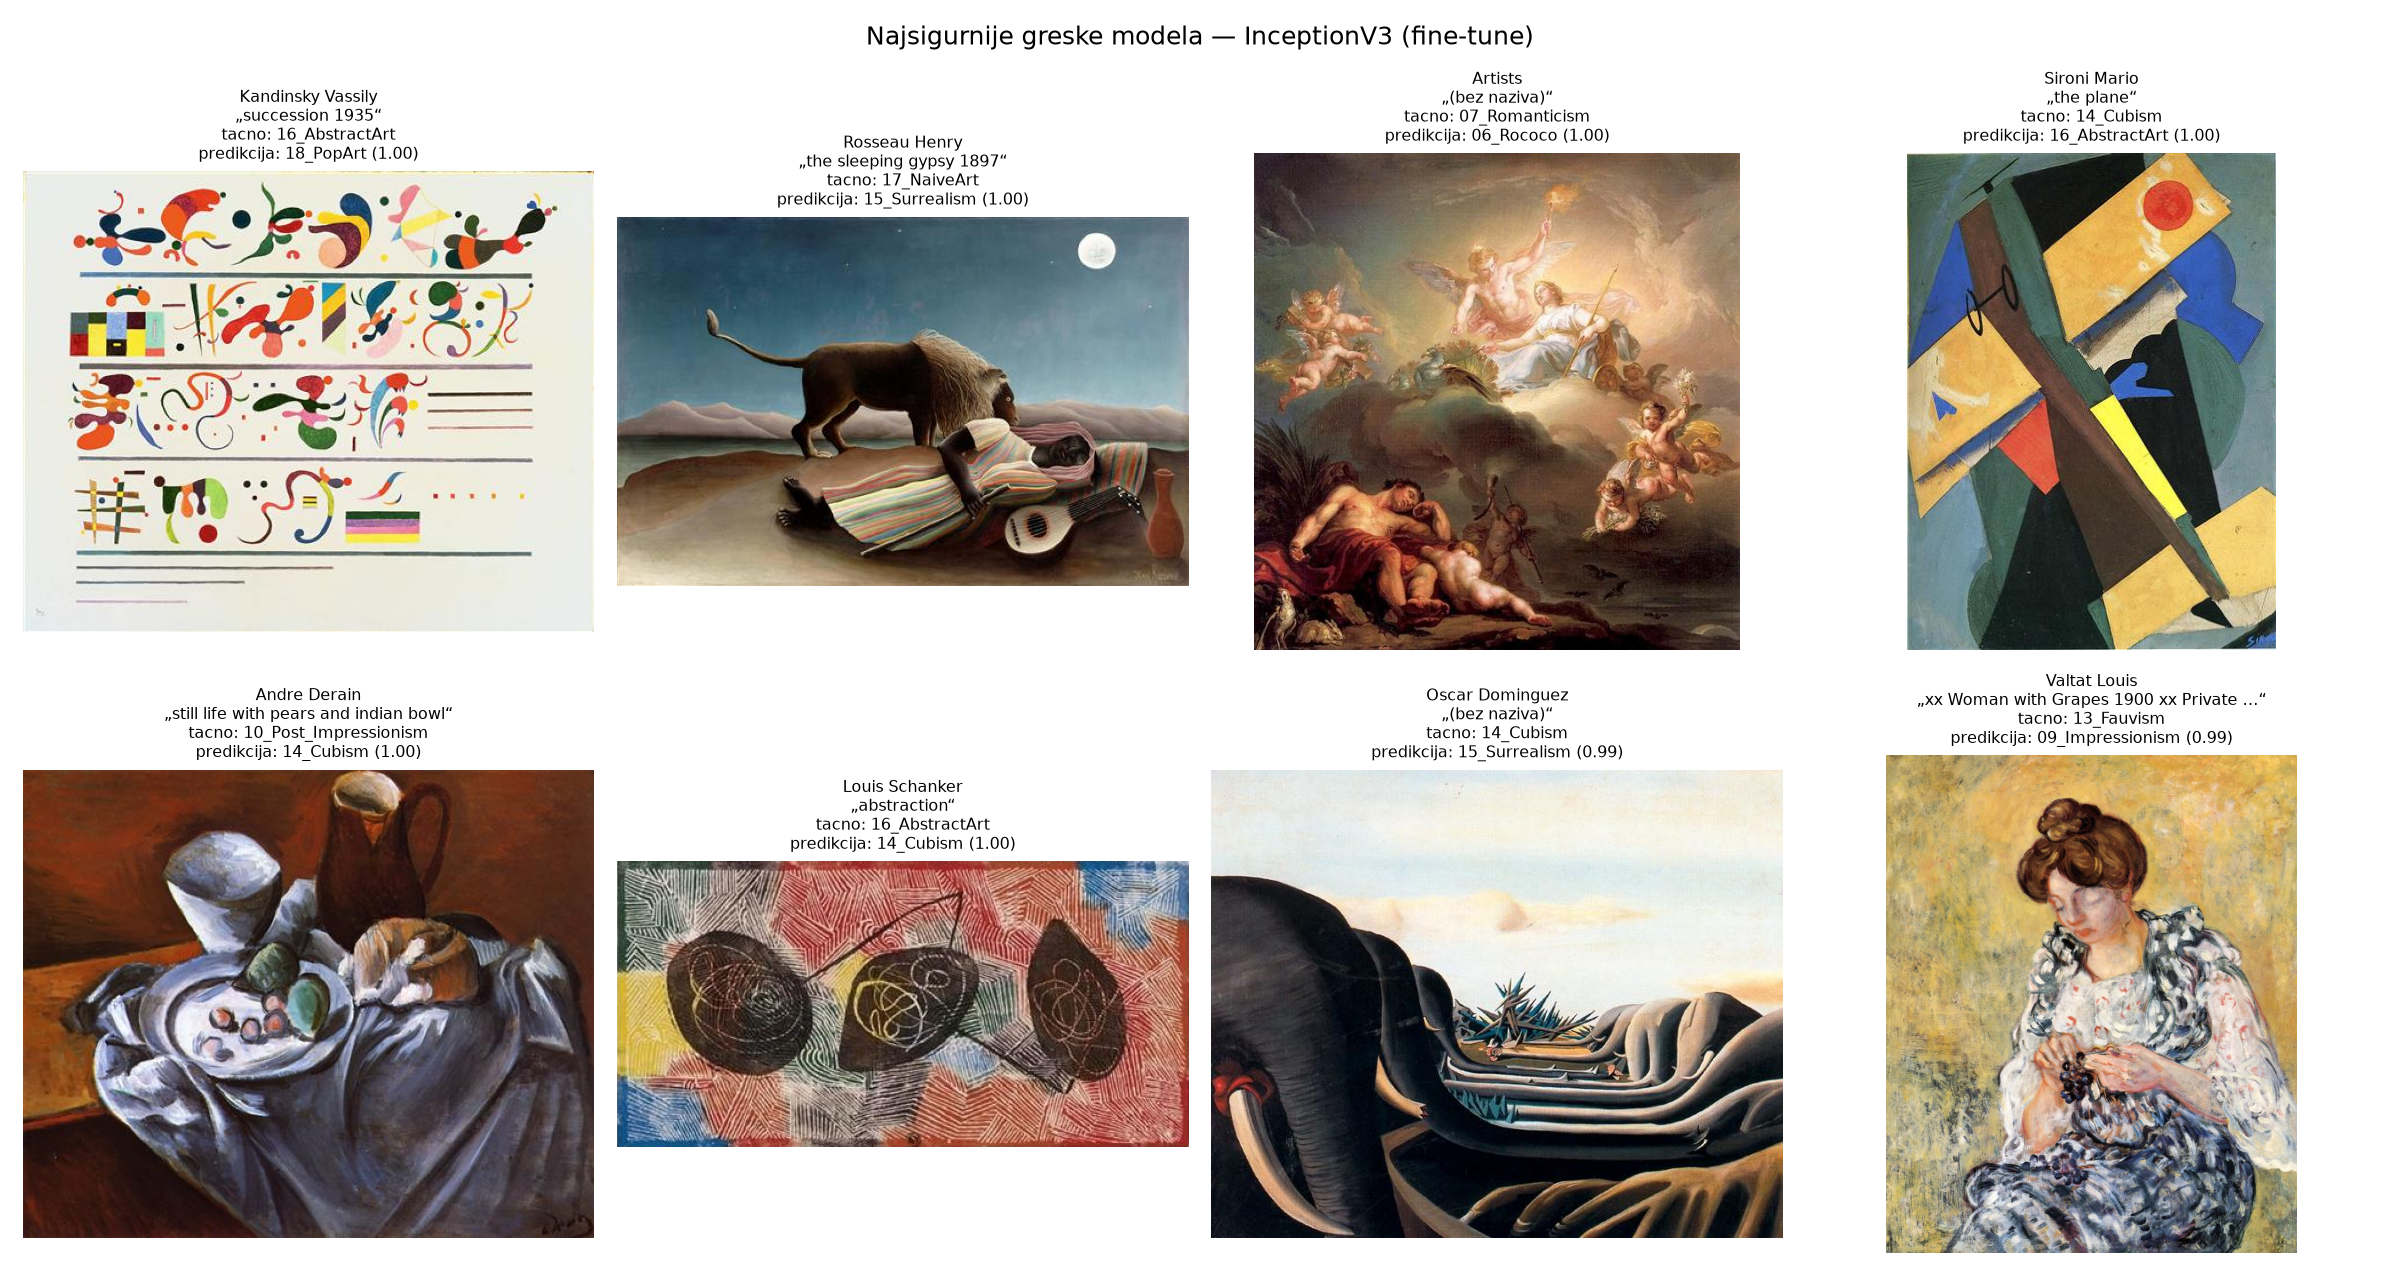
\includegraphics[width=\textwidth]{figures/transfer_finetune_errors.png}
  \caption{Primeri pogrešnih predikcija — transfer fine-tune}
  \label{fig:transfer_finetune_errorspng}
\end{figure}

Fine-tuning je podigao recall na teškim klasama (npr.\ surrealizam sa 36{,}6\% na 59{,}6\%).
Kod impresionizma recall pada, ali precision raste --- macro F1 je pouzdaniji pokazatelj od čistog recall-a.

\section{Diskusija}

Pretrenirana mreža daje mnogo bolje feature-e za ovaj zadatak nego učenje od nule na oko 12\,600 trening slika.
Hibridni model nije opravdao očekivanja zbog malog kapaciteta i istog broja epoha kao VGG-lite.
Fine-tuning poslednjeg bloka ima smisla jer ImageNet feature-i opisuju objekte i scene, a ne slikarski postupak.

\section{Zaključak}

Najbolji rezultat dao je InceptionV3 sa fine-tuningom: 56{,}91\% test accuracy i macro F1 0{,}570.
Transfer sa samo novom glavom ima 49{,}93\%. Custom VGG-lite stiže do 35{,}14\%, hibrid do 27{,}72\%.
Rezultat fine-tune modela uporediv je sa literaturom za isti skup.

\begin{thebibliography}{9}
\bibitem{florea2017}
C. Florea, C. Toca, F. Gieske.
\textit{Artistic Movement Recognition by Boosted Fusion of Color Structure and Topographic Description}.
IEEE WACV, Santa Rosa, CA, USA, 2017.

\bibitem{yu2017}
Y. Yu, O. Jin, D. Hsu.
\textit{Artistic Movement Recognition using Deep CNNs}.
Stanford University, CS231n, 2017.
\url{https://cs231n.stanford.edu/reports/2017/pdfs/411.pdf}

\bibitem{tfkeras}
TensorFlow / Keras dokumentacija: InceptionV3, ImageDataGenerator, transfer learning i fine-tuning.
\end{thebibliography}

\end{document}
